\graphicspath{ {imgs/} }
\documentclass[main.tex]{subfiles}
\begin{document}
\chapter{Methods}\label{chap:methods}
The following sections highlight the used methods and give a rough overview about the used tools. First the used environment of software tools is described. Then the theoretical concept of a Convolutional Neural Network is explained. A more extensive explanation to the different software packages and computational resources can be found in the appendix~\ref{app:software}.

\section{Software Packages}
Writing a program for solving the task of nodule detection with neural networks makes the use of certain frameworks necessary. Using Python as a versatile programming language allowed for writing code for all aspects of the project: from data preprocessing and training the network to analyzing the results. The language narrows down the number of frameworks available for training neural networks. For this thesis Tensorflow (\ref{appendix:tf}) was chosen since it is at the moment the most active framework (in the sense of implementation  Figure~\ref{fig:frameworks}). Other frameworks like Cafe, Theano and Keras would have been valid choices as well. The Sun Grid Engine of the institute is used for automated execution on several machines (see ~\ref{appendix:oge} for details) and was used for training the model.

\begin{figure}
\begin{center}
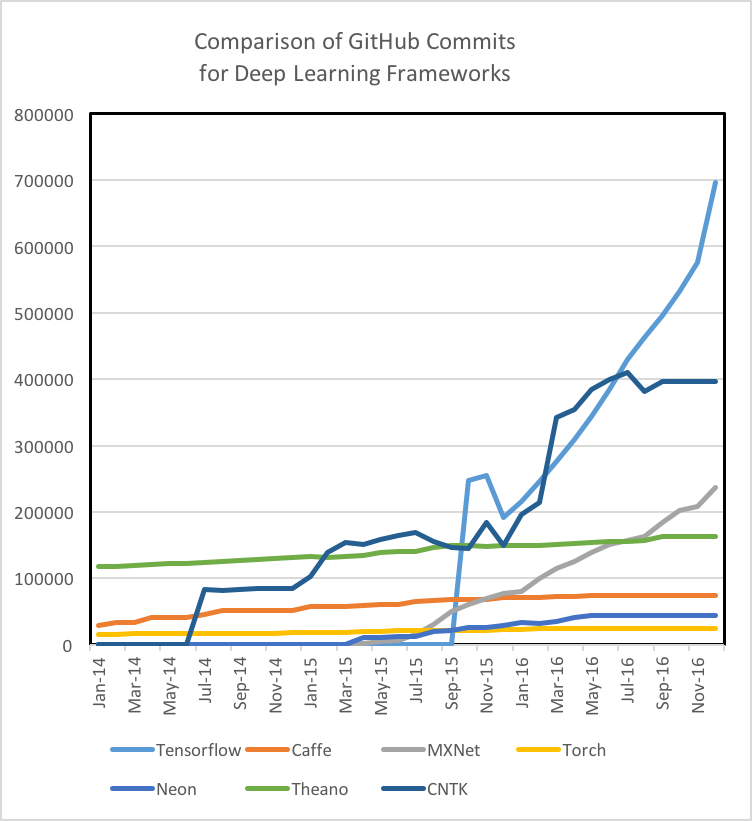
\includegraphics[scale=0.7]{deeplearning_frameworks.png}
\end{center}
\caption{Number of commits for the different deep learning frameworks. This figure is taken from Shapiro \cite{shapiro2017}.}
\label{fig:frameworks}
\end{figure}


\section{Convolutional Neural Network}
In this thesis a 3D Convolutional Neural Network (CNN) is used to classify the CT slices. The main motivation to use a 3D CNN in the case of nodule detection are the morphological features of the nodules that could not be fully utilized by a convolution that is only applied to 2D sections of the nodule. A CNN is similar to other artificial neural networks (ANNs) in the sense that it only uses forward connections, has an input and output layer and an arbitrary number of hidden layers in between. The hidden layers in a convolutional network are either convolutional or pooling layers which are in the end followed by one or more dense layers that perform the classification. Each of those layers is described in more detail in the following sections.

\subsection{Convolutional Layer}\label{ss:convlayer}
A convolutional layer consists of $1..n$ kernels that are represented through shared weights which are compared to classic convolution in computer vision not \emph{sliding} across the input but are duplicated across the image in a defined distance called stride. A stride of $2$ would for example mean that the kernel is convolved with every second pixel of the image. The convolution is applied in 3D which means that the filter kernels are also 3 dimensional and the stride is as well defined in all 3 directions of the input image $(x,y,z)$. A pixel in the output volume $y$ can be derived from an image $I$ with a 3D kernel $h$ of size $(2m+1,2n+1,2p+1)$ as described in equation~\eqref{eq:conv3d}.

\begin{equation}
y(x',y',z')=\sum_{i = -m}^{m}\sum_{j = -n}^{n}\sum_{k=-o}^{o} h(i+m,j+n,k+p) \cdot I(x+i,y+j,z+k) 
\label{eq:conv3d}
\end{equation}
 
As the layers of convolution stack the extracted features from the first layer are combined to more complex shapes.

\begin{figure}
\begin{center}
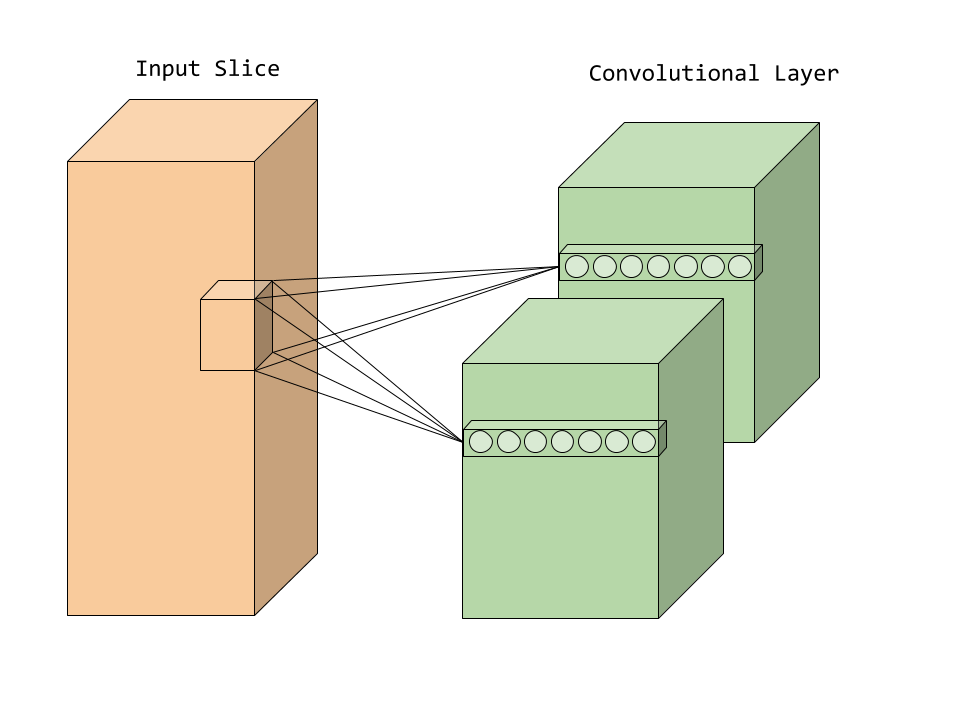
\includegraphics[scale=0.3]{conv_layer.png}
\end{center}
\caption{Structure of a convolutional layer. In image analysis the third dimension may encode the color informational, but in the example of Lung CT data it encodes additional spatial information. The figure shows two separate kernels that have shared weights for each kernel position in the input.}
\label{fig:conv_layer}
\end{figure}

The layers contain also a batch normalization step as described in \cite{ioffe2015batch} that was implemented in the Tensorflow layers class. batch normalization is scaling the activation of the layer to become normally distributed in each dimension of the features, but has additional parameters that can be learned to shift and scale these values again. This should bring several advantages like: reducing the dependence of the initialization method and allowing for higher learning rates. The batch normalization is followed by a max pooling layer which is applying a max filter to the normalized output. This adds additional small invariance to rotation and reduces the number of parameters in the network.


\subsection{Dense Layers}
The activation from the last convolutional layer is flattened into a $(1 \times n)$ vector and fed to the neurons of the fully connected layer. A neuron in this layer takes the weighted sum of the input and applies its activation function to it. In this network neurons with a rectified linear activation function are used, whose output is defined for an input $x$ and a number of weighted connections $w$ as:

\begin{equation}
\label{eq:dense}
y=max(\sum_w w \cdot x,0)
\end{equation}

This function is one of the standard activation functions in deeper architectures that avoid the vanishing gradient problem. This problem occurs when in the back propagation step the adaption of the weights is dependent on the repeated derivative of the activation function. For networks with several layers this leads to weight stagnation in the layers close to the input.


\end{document}
